%%%%%%%%%%%%%%%%%%%%%%%%%%%%%%%%%%%%%%%%%
% Beamer Presentation
% LaTeX Template
% Version 1.0 (10/11/12)
%
% This template has been downloaded from:
% http://www.LaTeXTemplates.com
%
% License:
% CC BY-NC-SA 3.0 (http://creativecommons.org/licenses/by-nc-sa/3.0/)
%
%%%%%%%%%%%%%%%%%%%%%%%%%%%%%%%%%%%%%%%%%

%----------------------------------------------------------------------------------------
%	PACKAGES AND THEMES
%----------------------------------------------------------------------------------------

\documentclass{beamer}

\mode<presentation> {

% The Beamer class comes with a number of default slide themes
% which change the colors and layouts of slides. Below this is a list
% of all the themes, uncomment each in turn to see what they look like.

%\usetheme{default}
%\usetheme{AnnArbor}
%\usetheme{Antibes}
%\usetheme{Bergen}
%\usetheme{Berkeley}
%\usetheme{Berlin}
%\usetheme{Boadilla}
%\usetheme{CambridgeUS}
%\usetheme{Copenhagen}
%\usetheme{Darmstadt}
%\usetheme{Dresden}
%\usetheme{Frankfurt}
%\usetheme{Goettingen}
%\usetheme{Hannover}
%\usetheme{Ilmenau}
%\usetheme{JuanLesPins}
%\usetheme{Luebeck}
\usetheme{Madrid}
%\usetheme{Malmoe}
%\usetheme{Marburg}
%\usetheme{Montpellier}
%\usetheme{PaloAlto}
%\usetheme{Pittsburgh}
%\usetheme{Rochester}
%\usetheme{Singapore}
%\usetheme{Szeged}
%\usetheme{Warsaw}

% As well as themes, the Beamer class has a number of color themes
% for any slide theme. Uncomment each of these in turn to see how it
% changes the colors of your current slide theme.

%\usecolortheme{albatross}
%\usecolortheme{beaver}
%\usecolortheme{beetle}
%\usecolortheme{crane}
%\usecolortheme{dolphin}
%\usecolortheme{dove}
%\usecolortheme{fly}
%\usecolortheme{lily}
%\usecolortheme{orchid}
%\usecolortheme{rose}
%\usecolortheme{seagull}
%\usecolortheme{seahorse}
%\usecolortheme{whale}
%\usecolortheme{wolverine}

%\setbeamertemplate{footline} % To remove the footer line in all slides uncomment this line
%\setbeamertemplate{footline}[page number] % To replace the footer line in all slides with a simple slide count uncomment this line

%\setbeamertemplate{navigation symbols}{} % To remove the navigation symbols from the bottom of all slides uncomment this line
}

\usepackage{graphicx} % Allows including images
\usepackage{booktabs} % Allows the use of \toprule, \midrule and \bottomrule in tables
\usepackage{multirow}
\usepackage{multicol}
\usepackage{adjustbox}
\usepackage{array}
\usepackage{tikz}
\usepackage{soul}
\usetikzlibrary{shapes.geometric, arrows, positioning, fit}
\usepackage[latin1]{inputenc}
\newcommand{\xmark}{\textcolor{red}{\text{\sffamily X}}}
\newcommand{\cmark}{\textcolor{green}{\checkmark}}
\newcommand{\tr}{\text{tr}}
\newcommand{\E}{\textbf{E}}
\newcommand{\diag}{\text{diag}}
\newcommand{\argmax}{\text{argmax}}
\newcommand{\argmin}{\text{argmin}}
\newcommand{\Cov}{\text{Cov}}
\newcommand{\Var}{\text{Var}}
\newcommand{\Vol}{\text{Vol}}
\newcommand{\bx}{\boldsymbol{x}}
\newcommand{\by}{\boldsymbol{y}}
\newcommand{\bX}{\boldsymbol{X}}
\newcommand{\bY}{\boldsymbol{Y}}
\sethlcolor{gray}
\makeatletter
\newcommand\SoulColor{%
  \let\set@color\beamerorig@set@color
  \let\reset@color\beamerorig@reset@color}
\makeatother
\definecolor{color1}{RGB}{128,13,13}
\definecolor{color2}{RGB}{70,128,13}
\definecolor{color3}{RGB}{13,128,128}
\definecolor{color4}{RGB}{70,13,128}

\newcommand{\faceA}{
\includegraphics[scale = 0.15]{face_photos/Amelia_Vega_0002.png}}
\newcommand{\faceB}{
\includegraphics[scale = 0.15]{face_photos/Jean-Pierre_Raffarin_0004.png}}
\newcommand{\faceC}{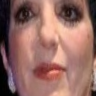
\includegraphics[scale = 0.15]{face_photos/Liza_Minnelli_0003.png}}
\newcommand{\faceD}{
\includegraphics[scale = 0.15]{face_photos/Patricia_Clarkson_0001.png}}

%tikz stufff


%----------------------------------------------------------------------------------------
%	TITLE PAGE
%----------------------------------------------------------------------------------------


%Extrapolating prediction error for 'extreme' multi-class classification

%with Rakesh Achanta and Yuval Benjamini

%'Extreme' classification refers to the classification with extremely
%large (on the order of millions) of labels, such as in photo or
%website annotation.  A natural question in these settings is whether
%the data is sufficiently rich to support high-accuracy classification
%with such a large label space.  Therefore, in this work, we address
%the question of predicting how well a classifier will scale with an
%increased number of classes, based on its performance in a smaller but
%representative classification problem. Under the assumption that the
%classes are sampled exchangeably, and under the assumption that the
%classifier is based on marginal probabilities (e.g. QDA or Naive
%Bayes), we derive a method for performance extrapolation based on
%unbiased estimation. We investigate the robustness of our methods to
%non-marginal classifiers in simulations and one optical character
%recognition example.


% Image sources
% http://sociable.co/social-media/how-to-disable-facebook-facial-recognition/
% https://alexanderskv.wordpress.com/2012/06/04/facial-recognition/
% https://medium.com/@ageitgey/machine-learning-is-fun-part-4-modern-face-recognition-with-deep-learning-c3cffc121d78#.fzgvan3ii

\title[Defense]{Supervised Evaluation of Representations}

\author{Charles Zheng} % Your name
\institute[Stanford] % Your institution as it will appear on the bottom of every slide, may be shorthand to save space
{Stanford University}
\date{\today} % Date, can be changed to a custom date

\begin{document}

\begin{frame}
\titlepage % Print the title page as the first slide
%(Joint work with Rakesh Achanta and Yuval Benjamini.)
\end{frame}

\section{Introduction}

%\begin{frame}
%\sectionpage
%\end{frame}


\begin{frame}
\frametitle{Overview}
\begin{center}
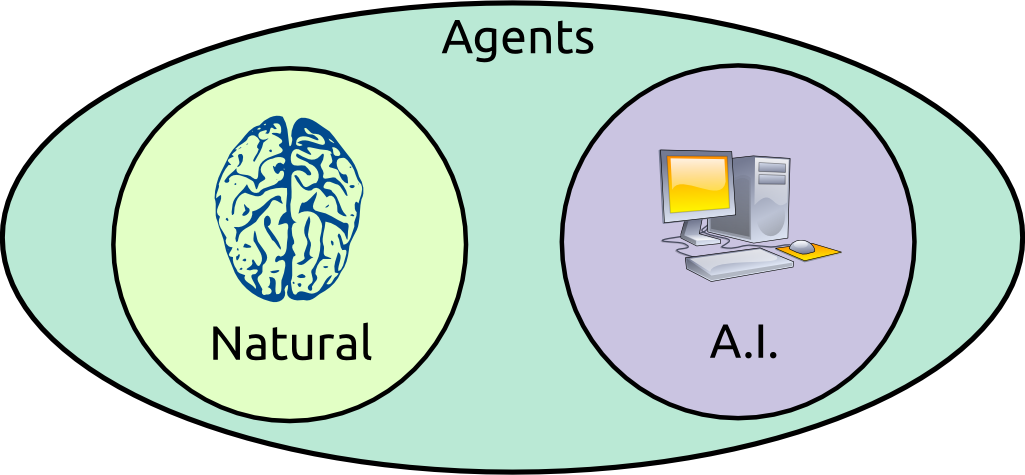
\includegraphics[scale = 0.3]{defense_diagrams/agents.png}
\end{center}
Human brains and machine learning algorithms tackle similar types of problems.
\end{frame}

\begin{frame}
\frametitle{Perception}
\begin{center}
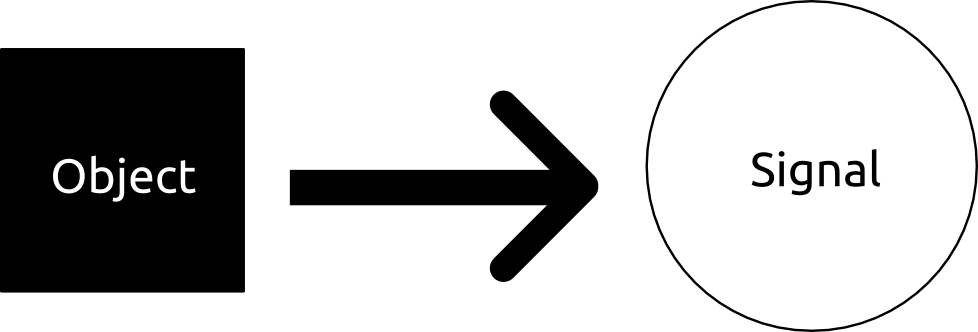
\includegraphics[scale = 0.4]{defense_diagrams/object_signal.png}
\end{center}
Perception: the problem of inferring \emph{objects} in the environment given observed \emph{signals}.
\end{frame}

\begin{frame}
\frametitle{Example: face recognition}
\begin{center}
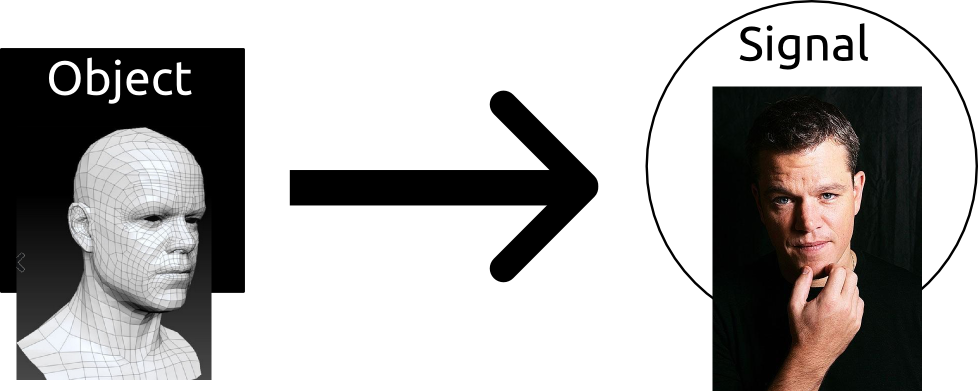
\includegraphics[scale = 0.4]{defense_diagrams/face_1.png}
\end{center}
\end{frame}

\begin{frame}
\frametitle{Perception}
\begin{center}
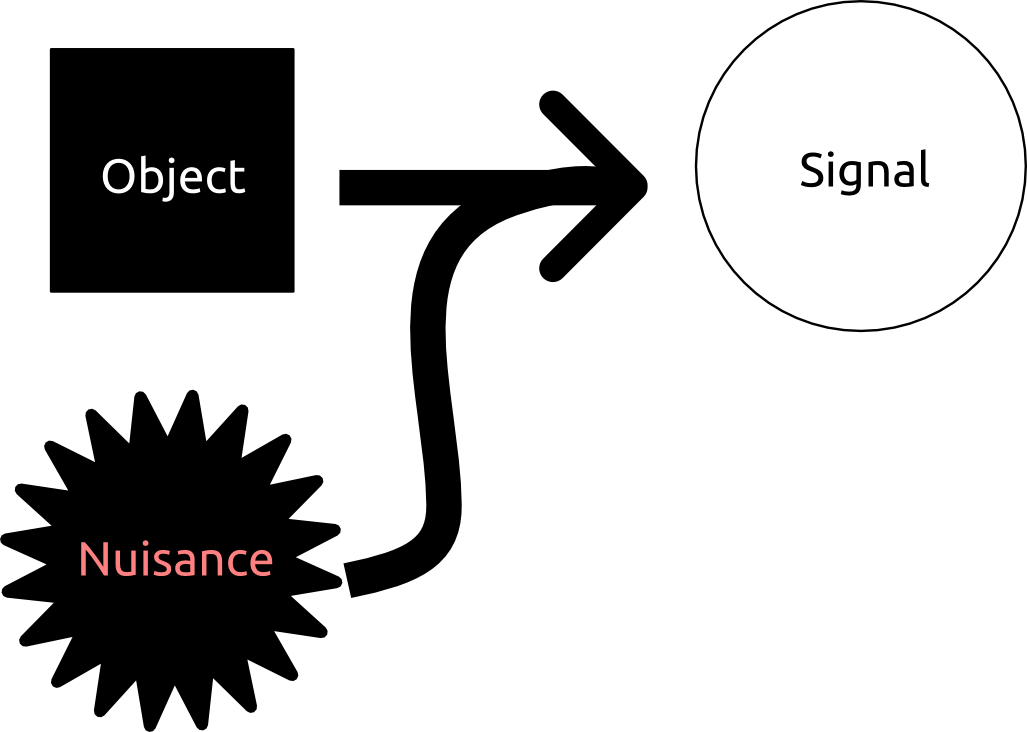
\includegraphics[scale = 0.2]{defense_diagrams/object_signal_nuisance.png}
\end{center}
The problem is complicated because there exist some \emph{nuisance parameters}, so the mapping from object to signal is not one-to-one.
\end{frame}

\begin{frame}
\frametitle{Example: face recognition}
\begin{center}
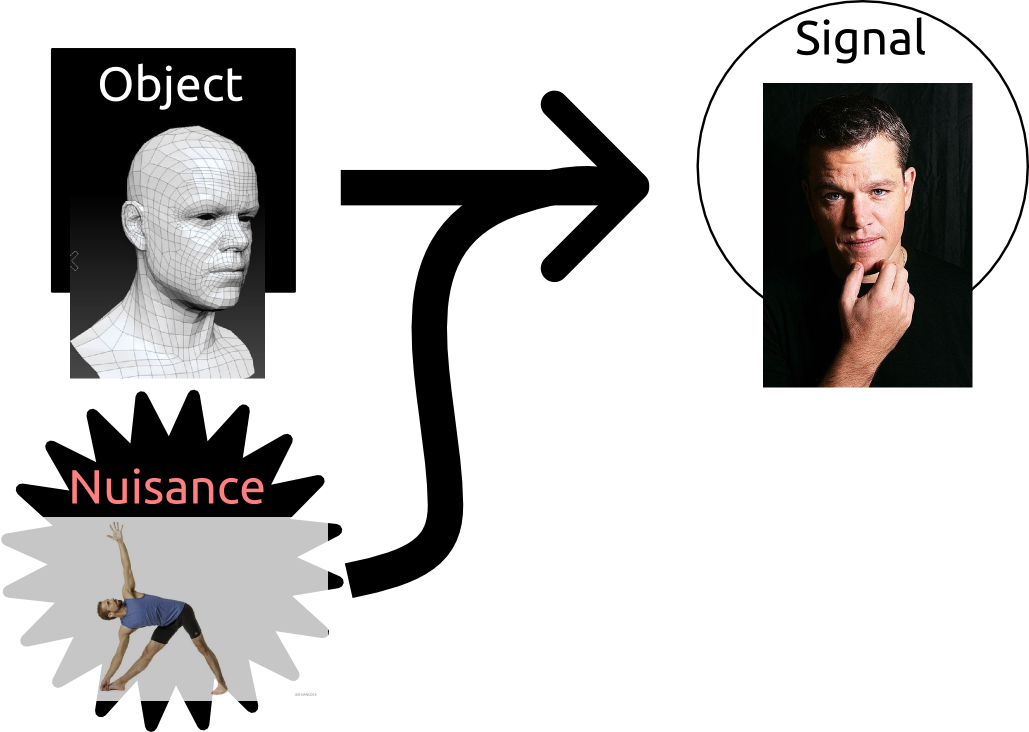
\includegraphics[scale = 0.2]{defense_diagrams/face_2a.png}
\end{center}
In face recognition, the \emph{pose} (including hairstyle) and \emph{lighting} are nuisance parameters.
\end{frame}

\begin{frame}
\frametitle{Example: face recognition}
\begin{center}
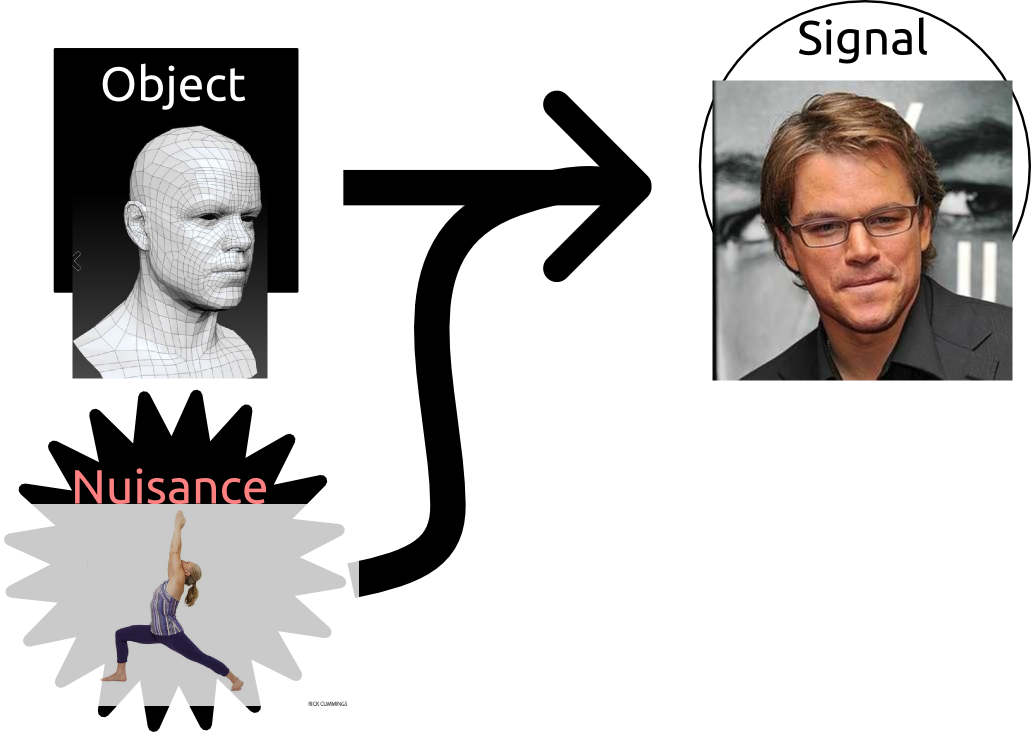
\includegraphics[scale = 0.2]{defense_diagrams/face_2b.png}
\end{center}
The same object can map to multiple signals.
\end{frame}


\begin{frame}
\frametitle{Perception}
\begin{center}
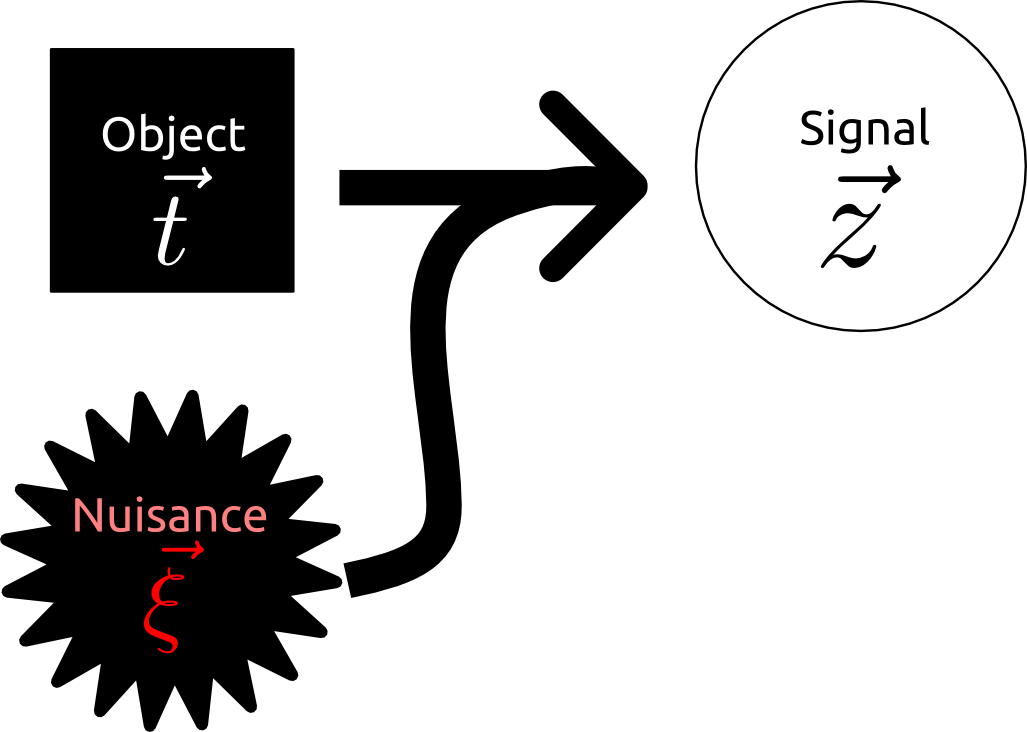
\includegraphics[scale = 0.2]{defense_diagrams/object_signal_nuisance2.png}
\end{center}
Assume there exists a function $\psi$ that maps objects and nuisance parameters to signals:
\[\vec{z} = \psi(\vec{t}, \vec{\xi}).\]
\end{frame}


\begin{frame}
\frametitle{What is a representation?}
\begin{itemize}
\item It is often hypothesized that \emph{complex objects} (images, sounds, etc.) can be mapped into a \emph{low-dimensional} space
\item A \emph{representation} is a nonlinear, dimensionality-reducing mapping
\end{itemize}
\end{frame}

\begin{frame}
\frametitle{Why do we care?}
\begin{itemize}
\item Application 1: Neuroscience.  Different regions of the brain have different representations of the same sensory stimuli.
\item Application 2: Machine learning.  A good representation leads to more accurate prediction.
\end{itemize}
\end{frame}

\begin{frame}
\frametitle{Example: Facial recognition}
\begin{itemize}
\item Used to tag images in software, security \pause
\item Preprocessing
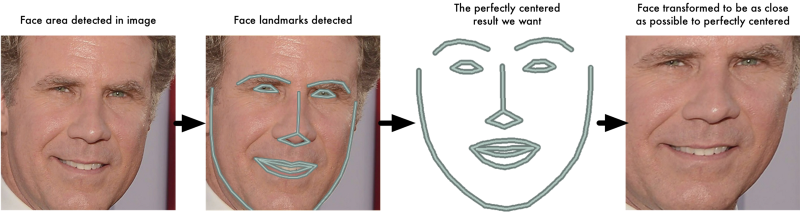
\includegraphics[scale = 0.4]{face_alignment.png}
\pause
\item Feature extraction
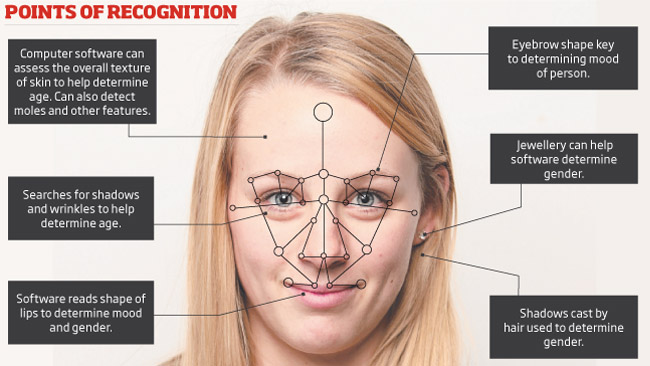
\includegraphics[scale = 0.4]{facerec_features.jpg}
\end{itemize}
\end{frame}

\begin{frame}
\frametitle{What defines a good representation?}

\end{frame}


\section*{Acknowledgements}

\begin{frame}
\sectionpage
\end{frame}

\begin{frame}
\begin{center}
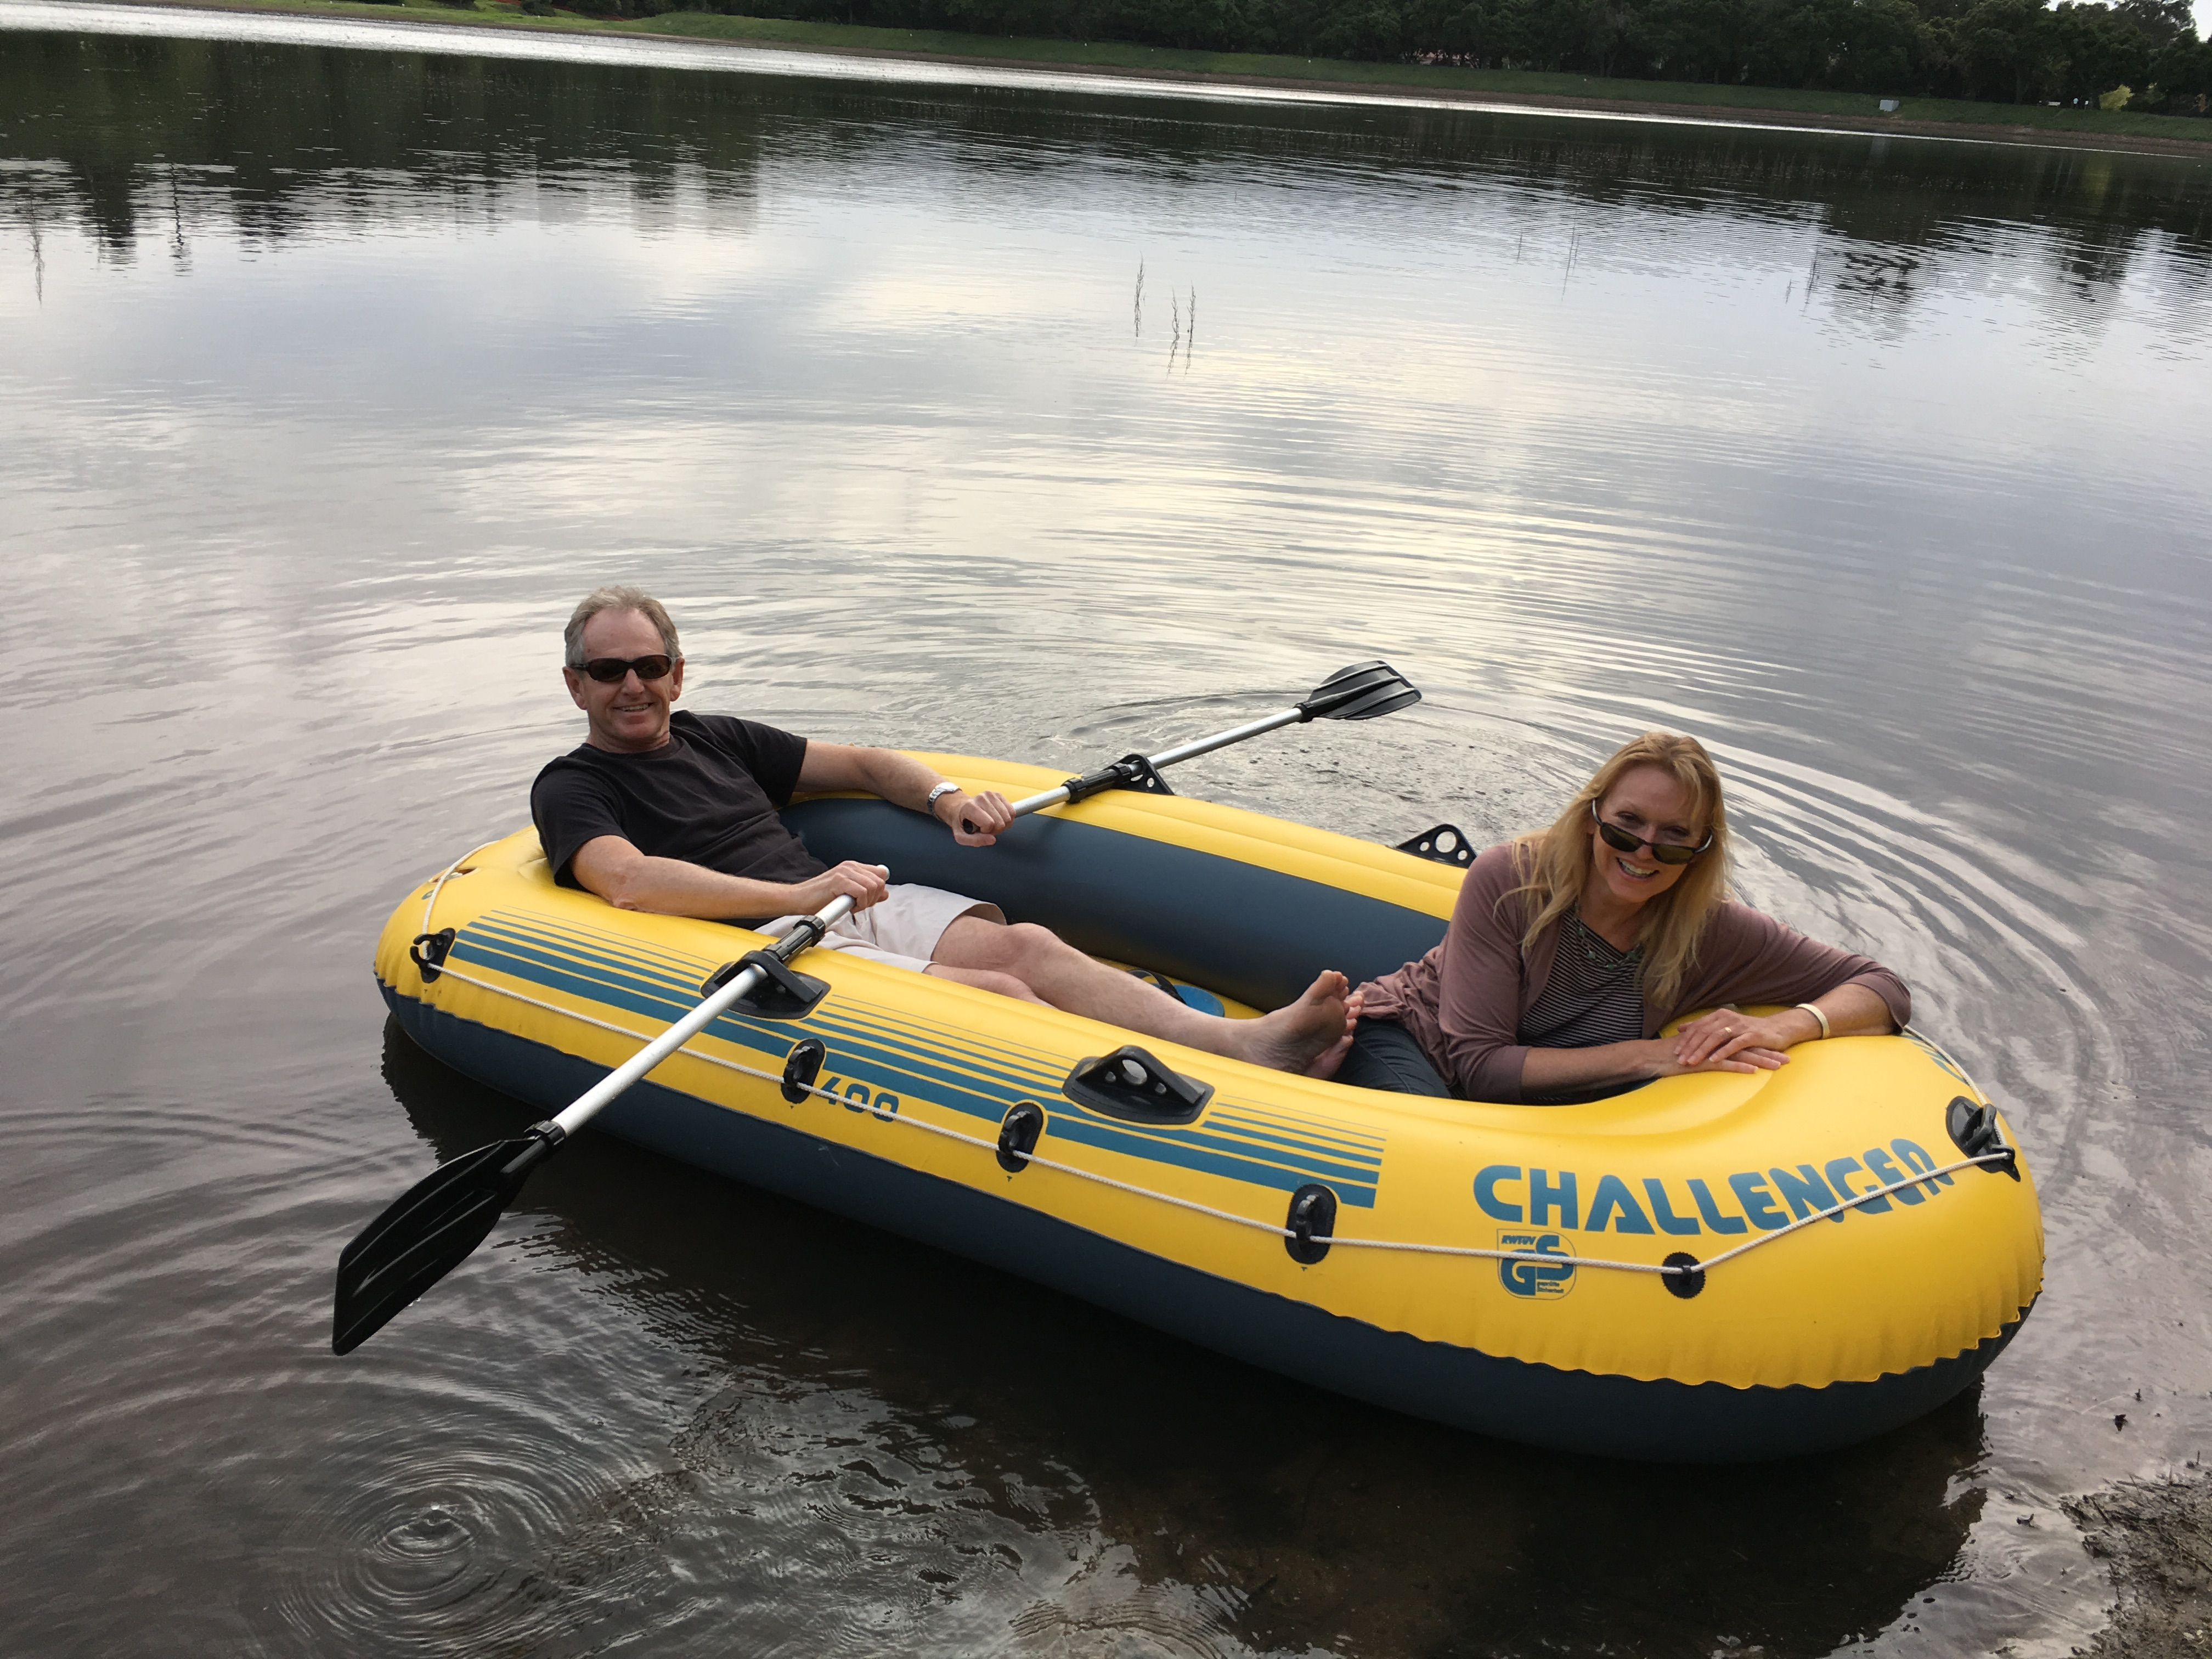
\includegraphics[scale = 0.04]{IMG_0703.JPG}

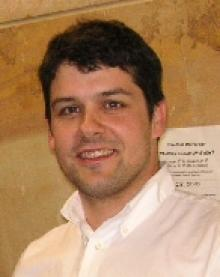
\includegraphics[scale = 0.6]{Taylor_2010.jpg}
\end{center}
\end{frame}

\begin{frame}
\begin{center}
\begin{tabular}{c}
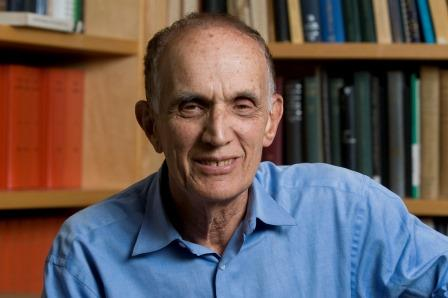
\includegraphics[scale = 0.7]{2014_Efron-indoors.jpg}\\
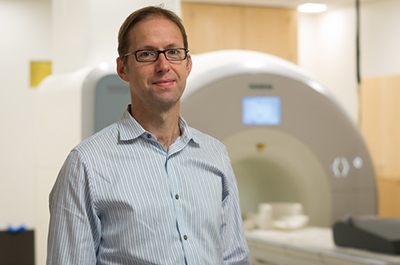
\includegraphics[scale = 0.16]{poldrack_photo2_400.jpg}\\
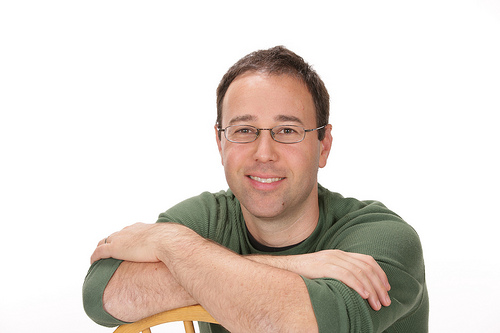
\includegraphics[scale = 0.16]{tsachypic.jpg}
\end{tabular}
\end{center}
\end{frame}

\begin{frame}
\begin{center}
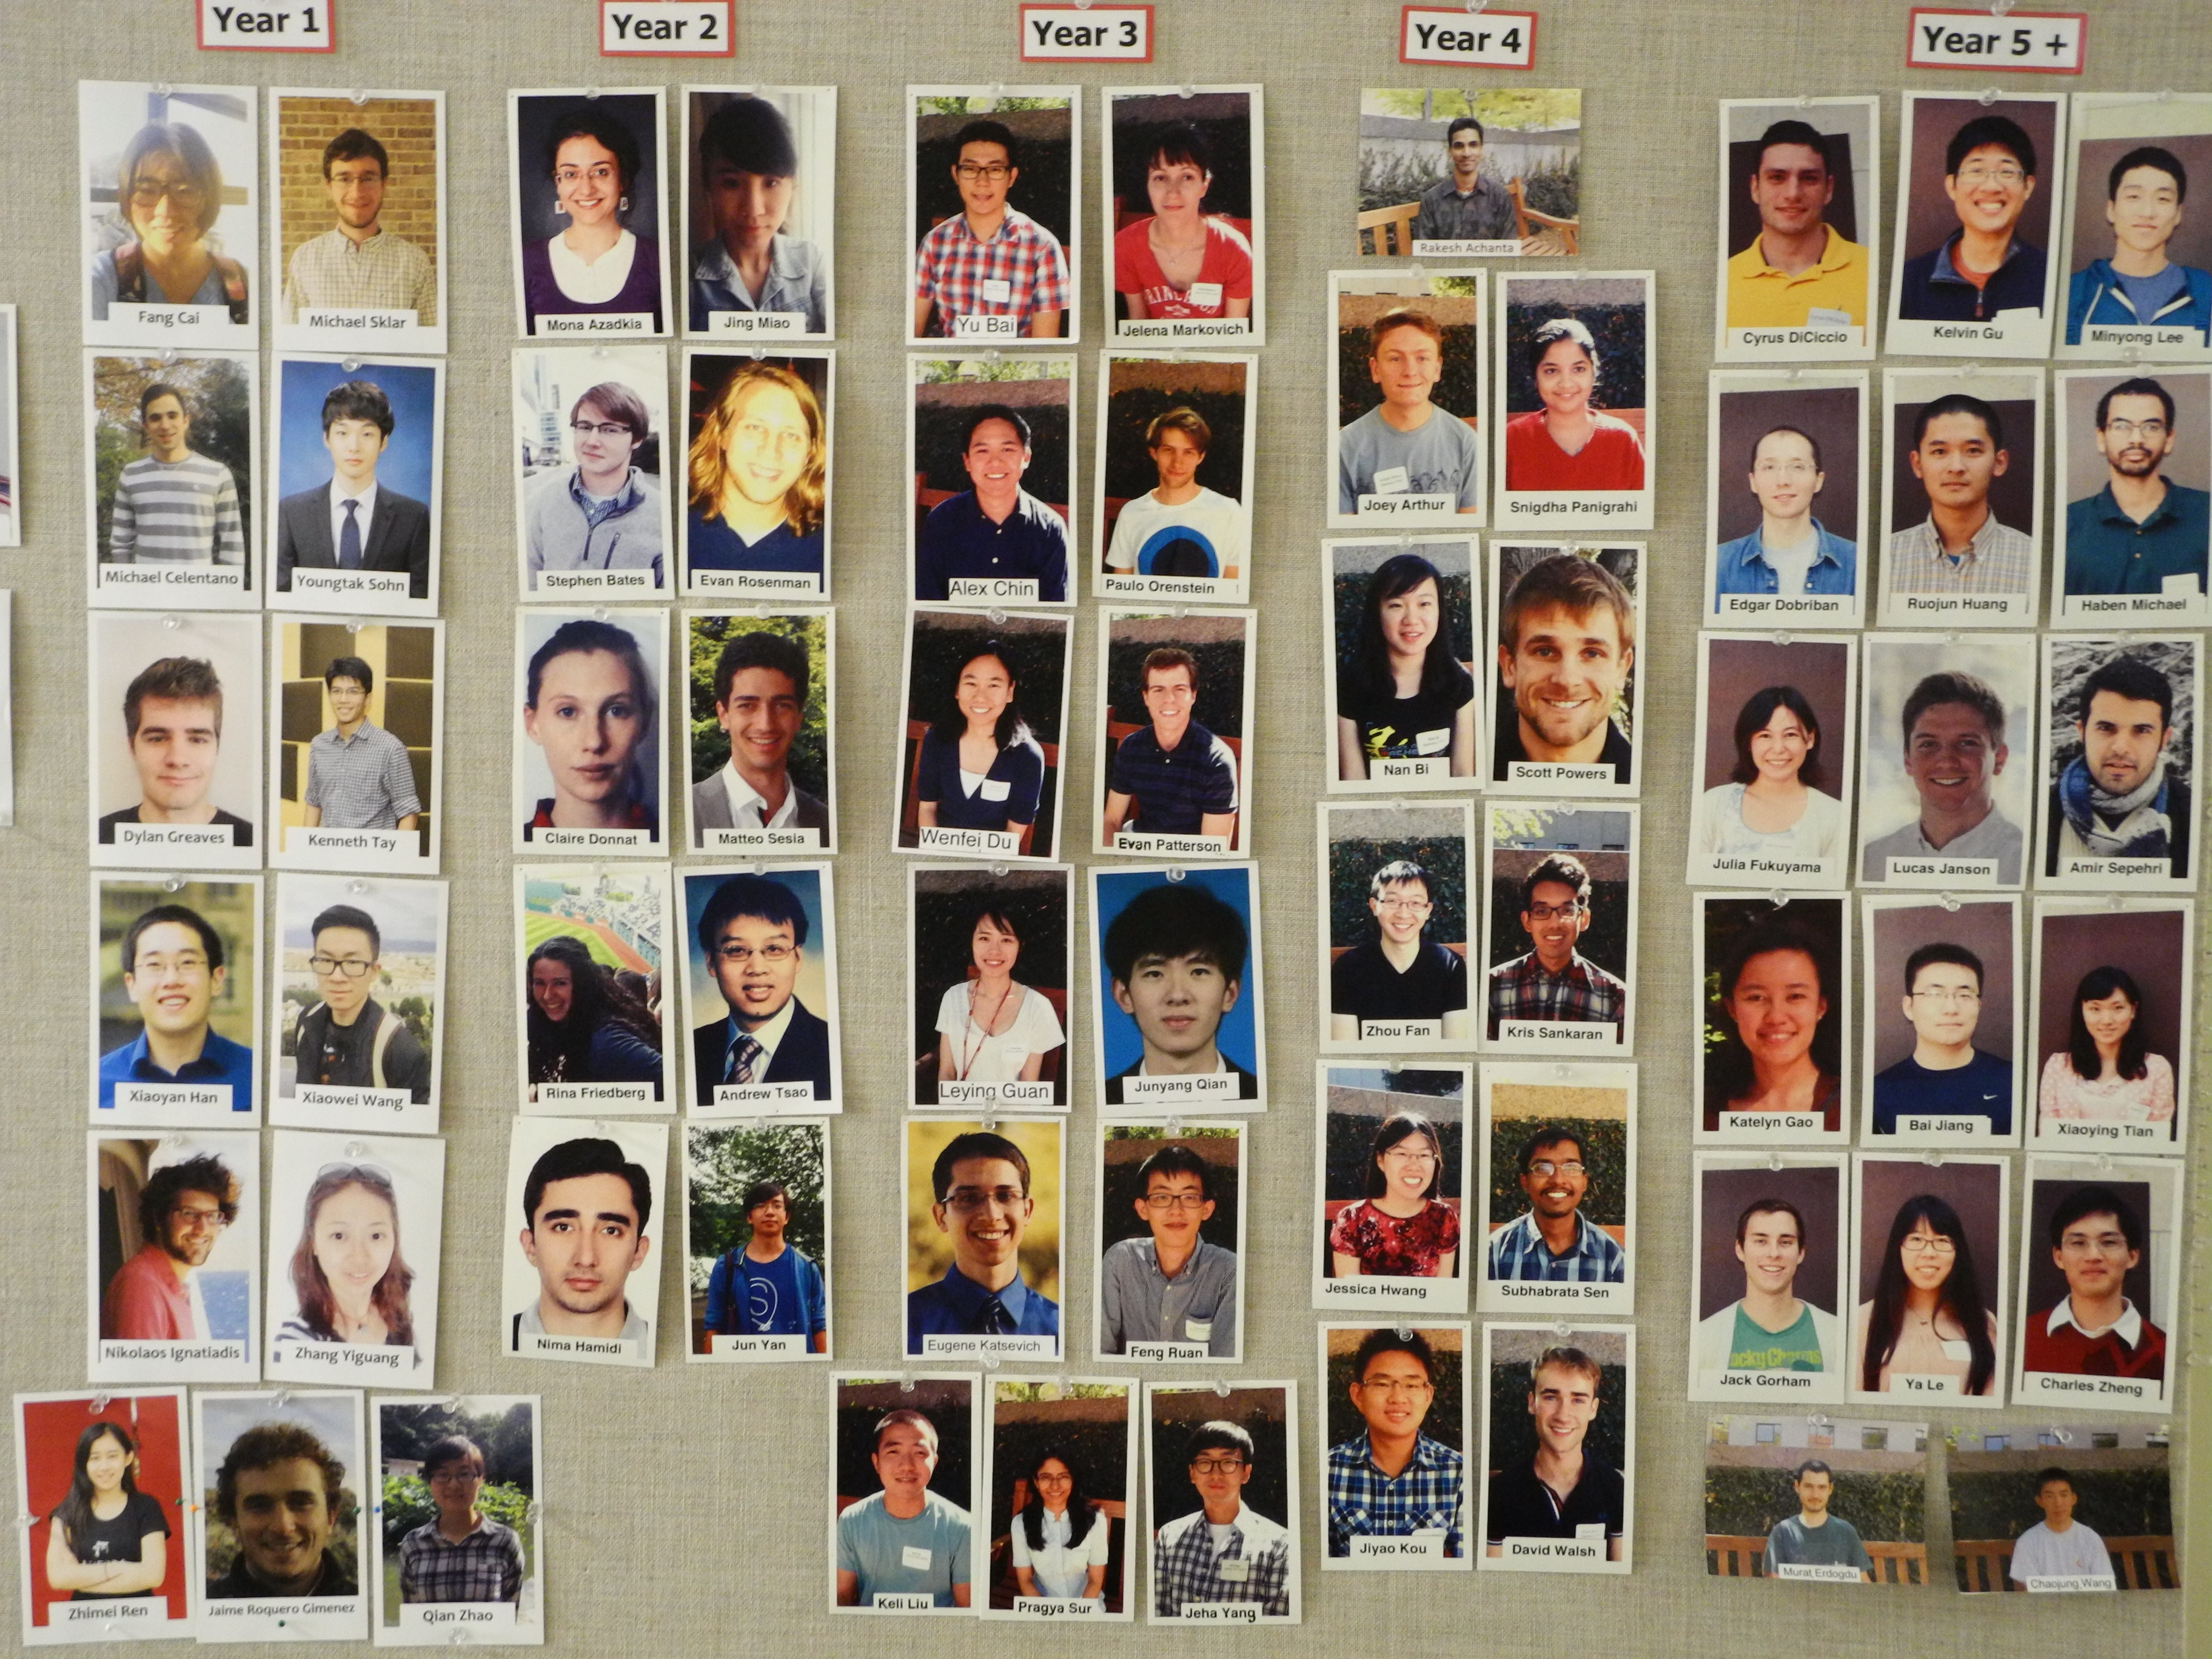
\includegraphics[scale = 0.3]{DSCN3964.JPG}
\end{center}
\end{frame}

\section*{The end}

\begin{frame}
\sectionpage
\end{frame}



\end{document}
\end{frame}
\end{document}


